%%%%%%%%%%%%%%%%%%%%%%%%%%%%%%%%%%%%%%%%%%%%%%%%%%%%%%%%%%%%%%%%%%%%%%%%%%%%%%%%
%2345678901234567890123456789012345678901234567890123456789012345678901234567890
%        1         2         3         4         5         6         7         8

\documentclass[letterpaper, 12 pt, conference]{ieeeconf}  % Comment this line out if you need a4paper

%\documentclass[a4paper, 10pt, conference]{ieeeconf}      % Use this line for a4 paper

\IEEEoverridecommandlockouts                              % This command is only needed if 
                                                          % you want to use the \thanks command

\overrideIEEEmargins                                      % Needed to meet printer requirements.

% See the \addtolength command later in the file to balance the column lengths
% on the last page of the document

% The following packages can be found on http:\\www.ctan.org
%\usepackage{graphics} % for pdf, bitmapped graphics files
%\usepackage{epsfig} % for postscript graphics files
%\usepackage{mathptmx} % assumes new font selection scheme installed
%\usepackage{times} % assumes new font selection scheme installed
\usepackage{amsmath} % assumes amsmath package installed
%\usepackage{amssymb}  % assumes amsmath package installed

\usepackage{graphicx}
\usepackage{cite}

\title{\LARGE \bf
Particle Filter for Skid-Steered Robot
}


\author{Rodolfo Corona$^{1}$ 
$~$ Chenyun Wu$^{2}$ $~$ Samer Nashed$^{3}$ $~$ Joydeep Biswas$^{4}$ %<-this % stops a space
% <-this % stops a space
\thanks{$^{1}$Rodolfo Corona is an undergraduate student at UT Austin who worked on this project as an REU student at UMass Amherst, he is responsible for the localization components of this project.}
\thanks{$^{2}$Chenyun Wu is a graduate student at UMass Amherst working under Dr. Subhransu Maji and conducted the vision related work for this project.}
\thanks{$^{3}$Samer Nashed is a graduate student at UMass Amherst working under Dr. Joydeep Biswas and served as Rodolfo Corona's graduate mentor for the project.}
\thanks{$^{4}$Joydeep Biswas is an Assistant Professor in the College of Information and Computer Sciences at UMass Amherst and served as Rodolfo Corona's faculty advisor for this project.} 
\thanks{*This work was supported in part by the NSF.}
%\thanks{$^{2}$Bernard D. Researcheris with the Department of Electrical Engineering, Wright State University,
%        Dayton, OH 45435, USA
%        {\tt\small b.d.researcher@ieee.org}}%
}


\begin{document}



\maketitle
\thispagestyle{empty}
\pagestyle{empty}


%%%%%%%%%%%%%%%%%%%%%%%%%%%%%%%%%%%%%%%%%%%%%%%%%%%%%%%%%%%%%%%%%%%%%%%%%%%%%%%%
\begin{abstract}

The ability to determine the location of a robot in its environment is a key requirement of autonomous robotics tasks. The particle filter algorithm, which may be used with various different combinations of sensors, is a common approach to this problem. Through the development of effective motion models for a skid-steered, outdoor robot, we have implemented a particle filter which may be used to test the effectiveness of a variety of sensors. Having tested the algorithm with a combination of odometry and GPS, we will explore methods from computer vision, such as convolutional neural networks (CNNs), for effectively incorporating video cameras as sensors. To this end, we have collected a data set of images mapped to locations on a variety of maps which vary in size and path complexity, something which will allow us to test both the efficacy and robustness of the methods we will explore.

\end{abstract}


%%%%%%%%%%%%%%%%%%%%%%%%%%%%%%%%%%%%%%%%%%%%%%%%%%%%%%%%%%%%%%%%%%%%%%%%%%%%%%%%
\section{INTRODUCTION}
For an autonomous robot to operate effectively in its environment, it is necessary that it be able to track its location over time. More formally, \textbf{localization} may be defined as the task of determining a robot's \textbf{pose}, which is of the form $(x~y~\theta)^T$ and denotes a robots location and orientation within a given map $M$. Although simple to define, this task is made difficult by the inherently noisy nature of sensors. Even if a particular sensor's error is small, the dependence of each reading on the previous ones can quickly give rise to large systematic errors.  
\par
In order to combat this problem, localization algorithms often require and are greatly aided by the use of multiple sensors. By getting location estimates from a variety of sources, a tighter probability distribution for a robot's pose may be computed, allowing the error and uncertainty in pose estimates to be mitigated. 
\par
In this paper we detail the implementation of a \textbf{particle filter}, a popular localization algorithm, for use with the Jackal, a skid-steered, outdoor robot developed by ClearPath Robotics\footnote{https://www.clearpathrobotics.com/jackal-small-unmanned-ground-vehicle/}. Furthermore, we derive a motion model for the robot and employ the use of GPS sensors as well as its internal odometry for our implementation.

\begin{figure}[h]
\centering
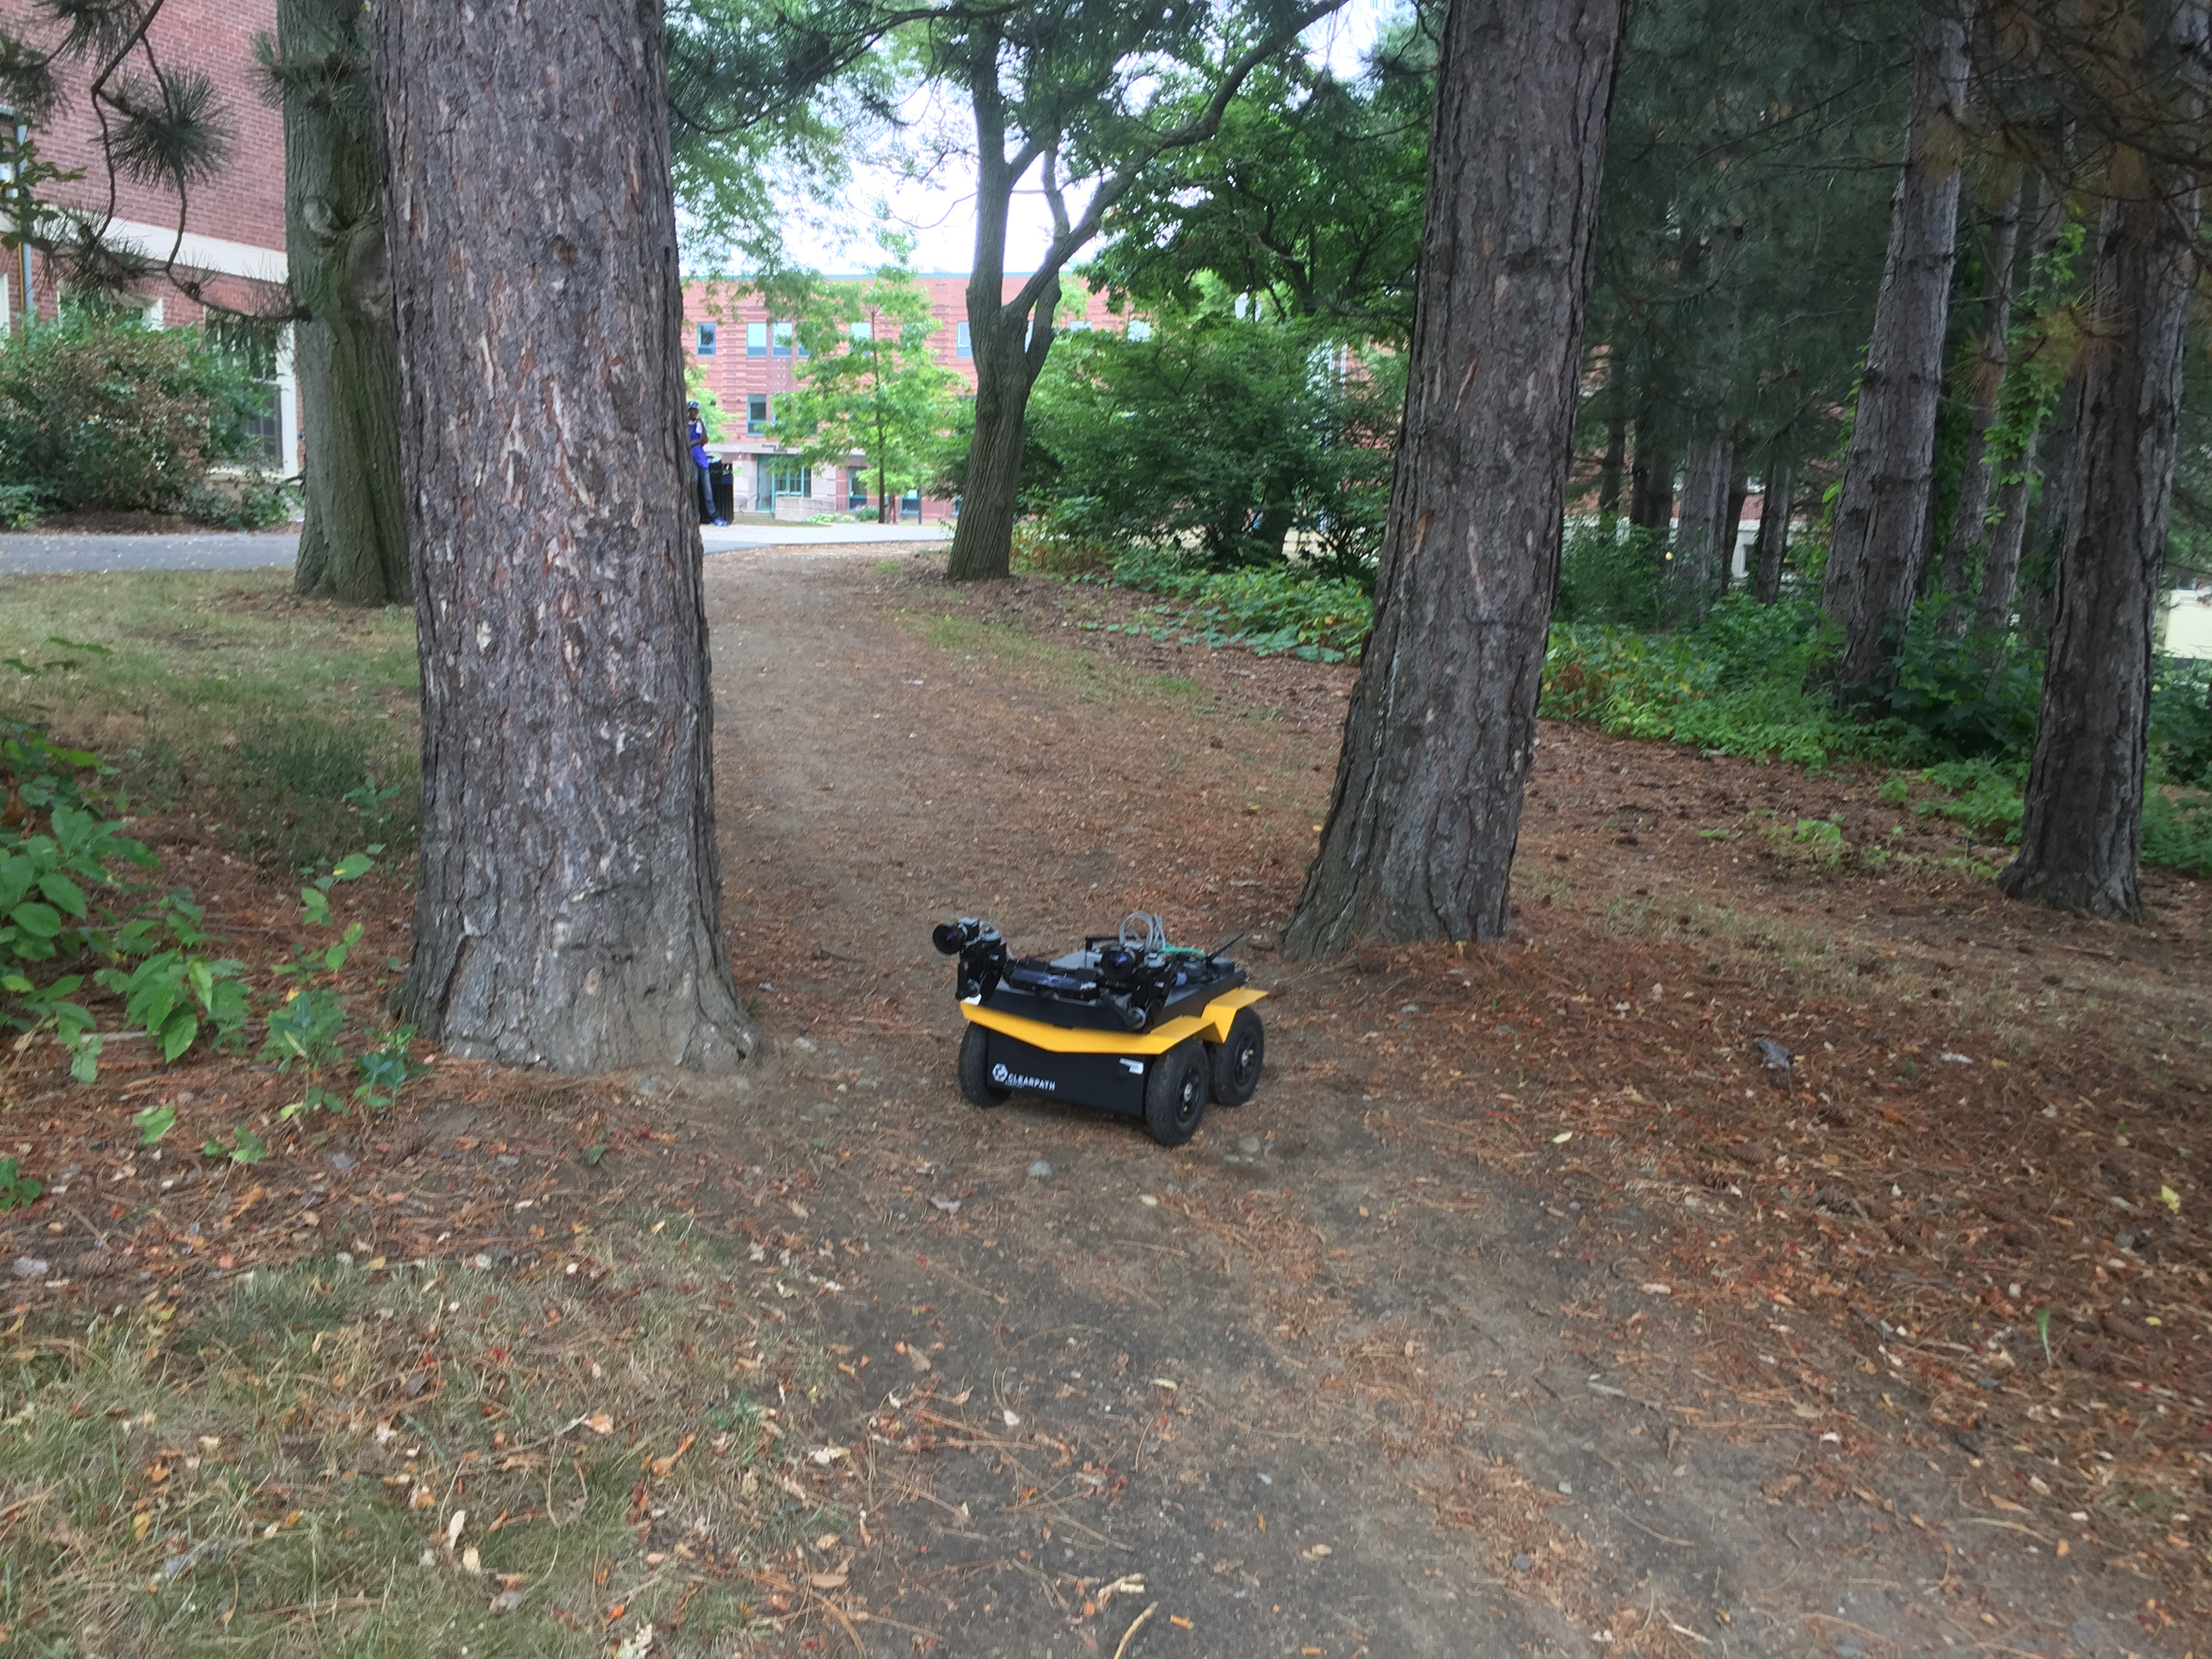
\includegraphics[scale=0.07]{JackalPose}
\caption{The ClearPath Jackal equipped with two fish-eye camera lenses.}
\end{figure}

\par 
This work also explores how cameras may be used as sensors for localization. In order to map images to pose estimates, we use convolutional neural networks (CNNs) to extract high-level feature vectors from images, which are then experimented with using a variety of different classification algorithms. 

\section{Background}
\subsection{Localization}
The task of any localization algorithm is to determine a likely estimate for a robot's current pose $(x~y~\theta)^T$. In order to accomplish this, the algorithm must work effectively with readings from its ensemble of sensors \cite{thrun2002robotic}. 
\par
At each time step $t$, a robot receives a \textbf{control} $u_t$, and a \textbf{sensor reading} $z_t$. The control is an estimate of the robot's translation and rotation since the last time step as given by its internal sensors, such as odometry and IMU (inertial measurement unit), and is of the form $(\Delta x~\Delta y~\Delta \theta)^T$. Similarly, the sensor readings come from sensors external to the robot, such as GPS or laser range finders, and give a pose estimate of the form $(x_z~y_z~\theta _z)^T$. 
\par 
Using these readings, the robot's most likely pose $\textbf{x}_t=(x_t~y_t~\theta _t)^T$ may be found using the following formula: 
$$
\textbf{x}_t = argmax_{\textbf{x}}~P(\textbf{x}|\textbf{x}_{0:t-1}, u_{0:t}, z_{0:t})
$$
Given that the space of possible poses is continuous, however, makes the task of searching through it intractable. Further, the cost of computing such a function can quickly grow too large because of the dependence of the estimate on all previous estimates and readings. 
\par
In order to combat the growth of the cost, the \textbf{Markov assumption} may be used, allowing us to compute an estimate using only the current time step's readings and the previous time step's pose estimate:
$$
\textbf{x}_t = argmax_{\textbf{x}}~P(\textbf{x}|\textbf{x}_{t-1}, u_t, z_t)
$$
\par
For working tractably in a continuous space, localization algorithms use a variety of methods to approach this function. The most common strategy is to assume that the control and sensor readings are independent from each other and split the function into two statistical models, the \textbf{motion model} and the \textbf{perceptual model}. The motion model approximates the probability distribution $P(\textbf{x}_t|\textbf{x}_{t-1},u_t)$ using the control reading and noise generated from experimentally derived distributions such as Gaussians. The perceptual model approximates the probability distribution $P(\textbf{x}_t|z_t)$ using experimentally derived distributions to model sensor uncertainty. In general, the motion model is used in order to estimate the trajectory of the robot over time. Given the dependence of each motion model estimate on the previous time step's estimate, the motion model is highly prone to systematic errors. The perceptual model is therefore used in order to bias this trajectory estimate and keep the error in check. 

\subsection{Particle Filters}

The approach of the particle filter algorithm to the problem of tractability is to use a discrete set of $N$ random variables known as \textbf{particles}. At each time step, particles are assigned different pose estimates based on the robot's models. This distribution of particles is then used in order to approximate the true probability distribution of the robot's pose. 
\par
To accomplish this, the algorithm iterates through three main procedures at each time step. Firstly, each particle's pose estimate is computed using its previous pose and the current control readings in the \textit{elapse time} step. Following this, the \textit{weighing} step uses the current sensor reading in order to assign weights to each particle's estimate. Finally, in the \textit{resampling} step, a probability distribution of possible poses is computed based on the particle poses and weights, which is used to re-sample the particles' poses. 

\subsubsection{Elapse Time}
At each time step $t$ the robot's motion model is used in conjunction with the current control reading $u_t$ in order to derive a new pose for each particle:
\begin{align*}
\textbf{x}_t = \begin{bmatrix}
				x_t \\
				y_t \\
				\theta _t
				\end{bmatrix} 
				=
				\begin{bmatrix}
				x_{t-1} + x_u + \epsilon _x\\
				y_{t-1} + y_u + \epsilon _y\\
				\theta _{t-1} + \theta _u + \epsilon _\theta				
				\end{bmatrix}
\end{align*}
Where $\epsilon$ represents an error reading sampled from an experimentally approximated distribution for each of the three dimensions. 
\subsubsection{Weigh}
Immediately after receiving a pose estimate, each particle is assigned a weight based on the current sensor model reading $z_t$.  
\subsubsection{Resample} 
Using each of the $N$ particles' weight, a discrete probability density function of pose estimates is built such that the probability of any particle's pose estimate is proportional to its weight: 
$$
\forall _{1\leq i \leq N}~P(\textbf{x}^i)=\frac{w_i}{\sum _{i=1} ^N w_i}
$$
Where $\textbf{x}^i$ and $w_i$ denote the $i$-th particle's pose estimate and weight. Each particle's pose estimate is then re-sampled using this distribution, which results in the particle distribution being concentrated around the most likely robot locations.  

\subsection{Convolutional Neural Networks}

A neural network (NN) is a model used for machine learning which represents a funciton $f:X\to Y$ of datum to labels. Generally, these models are used in order to classify data in tasks such as object recognition in images. 
\par
In order to do this, a network takes a vector or tensor representation of data \textbf{x} as input (such as $W\times H \times 3$ matrix for an image of dimensions $W\times H$ and RGB color channels) and performs a set of transformations on it to generate its output. Each \textbf{layer} of a network consists of a set of \textbf{neurons}, with neurons at different layers connected to each other. Every neuron is assigned a weight vector, the weights of which must be learned using machine learning techniques, with each weight corresponding to each of its inputs from the previous layer.  

\begin{figure}[h]
\centering
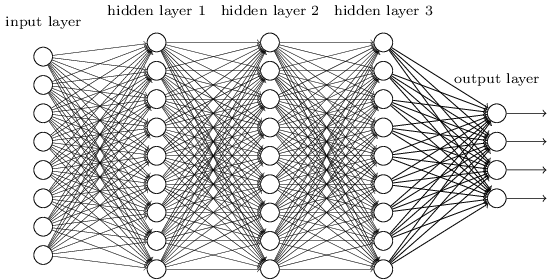
\includegraphics[scale=0.43]{neural_net}
\caption{A fully connected, feed-forward neural network. Neurons are connected to each neuron in the previous and next layers. Image source: http://neuralnetworksanddeeplearning.com/chap6.html}
\end{figure}

At each layer, a neuron will compute the dot product between its input vector and its weight vector, the result of which is then fed to the neurons at the next layer to which it is connected to. In more concrete terms, the model performs a matrix multiplication at each layer in order to derive its output. This basic neural network model is known as a \textbf{feed forward} architecture and is also generally implemented as a \textbf{fully connected} model in which the neurons in each layer will be connected to all of the neurons in the next. 
\par
It may be observed that as the size of images grows, the number of weights that must be learned in a network can quickly become intractable. Due to the growth in learned parameters, the amount of training data required may also become infeasible. Furtheremore, at least in the case of images, much of the inputted information is redundant and need not all be processed for effective classification. Convolutional neural networks alleviate this problem by employing the use of \textbf{convlutional} and \textbf{pooling} layers in their architecture.
\par
Instead of taking as input the entirity of an image, neurons in a convolutional layer will instead receive small patches, such as $3\times 3$ patches, and convolve the values in each pixel using a \textbf{kernel function}. A kernel function used within a neuron is known as a \textbf{filter} because each kernel function is constructed to reflect the presence of different types of features in a patch, such as edges, corners, or colors. In other words, neurons in a convolutional layer will output higher values, or become "activated", when they detect the presence of certain features. 
\par
Neurons in a pooling layer will take input from neurons in convolutional layers and perform some form of downsampling on their input, which reduces the dimensionality of its output which results in a lower number of weights going forward. Similarly to the convolutional layers, neurons in this layer will be activated by the presence of certain features in the input, but are invariant to the order of the input. 
\par
Finally, the fully connected layers of a CNN work identically to those of a fully connected network, and are generally used as the last layers in order to compute a final classification for the given input. 
\par

\begin{figure}[h]
\centering
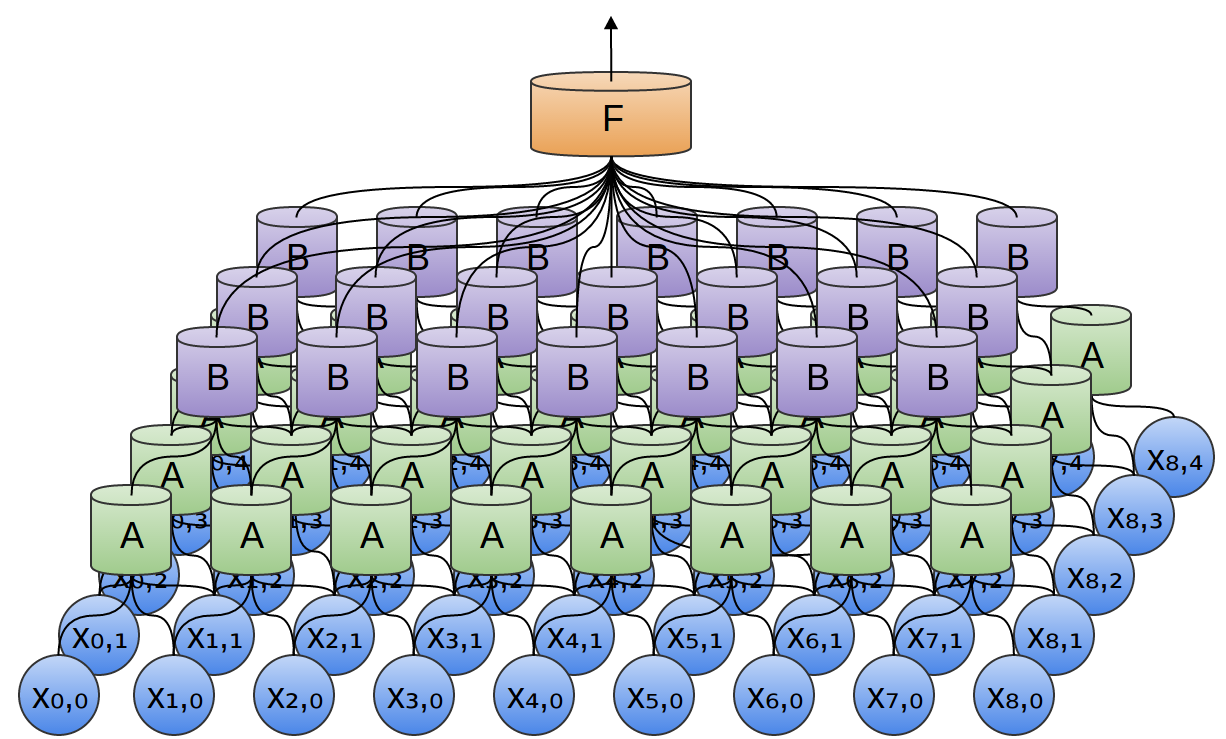
\includegraphics[scale=0.15]{cnn}
\caption{A convolutional neural network. The number of learned parameters is greatly reduced compared to fully connected architectures through the use of convolutional and pooling layers. Image source: http://colah.github.io/posts/2014-07-Conv-Nets-Modular/}
\end{figure}

At a high level, the network may be thought of as finding certain features in specific patches in the convolutional layers. The pooling layers may be thought of as seeking out only the presence of these features among groups of patches, indifferent to which patch. As the input travels through the network, the types of features which are computed also become more abstract, taking the form of fuller patterns or even representing partial objects themselves. 
\par
Although a lower level description of CNNs is beyond the scope of this work, a more in depth treatment of the subject matter may be found at \cite{deeplearningbook, AlexNet}. 
 

\section{Related Work}

There has been much work done on indoor robot localization. In indoor localization environments, the evnironment remains mostly static and does not vary in factors such as weather, lighting, and obstacle locations. The presence of walls also makes it much easier to use sensors such as laser-range finders. 
\par
Outdoor localization, however, is complicated by many factors which can vary greatly based on time of day and season, amongst other things. Irie et al. propose a solution to this problem which uses stereo cameras in order to generate 2D point clouds of the environment \cite{irie2010mobile}. This method is used during data collection to create a global grid map of the robots environment. During localization, these point clouds are used in two ways. Firstly, the motion of the robot is estimated at each timestep using the changes in point clouds, something which serves as the motion model for their particle filter implementation. As a perceptual model, they try to evaluate the local point cloud  to the global map that was generated during data collection. They claim that their methods are more resilient to changes in lighting than other approaches.
\par
Similarly to Irie et al., Agrawal et al. use the Harris corner detection method \cite{Harris} along with stereo cameras in order to calculate movement between timesteps to serve as a motion model \cite{agrawal2006real}. Instead of using vision as a perceptual model, however, they use GPS sensors. Additionally, they implement a Kalman Filter for localization \cite{Kalman}.

\begin{figure}[h]
\centering
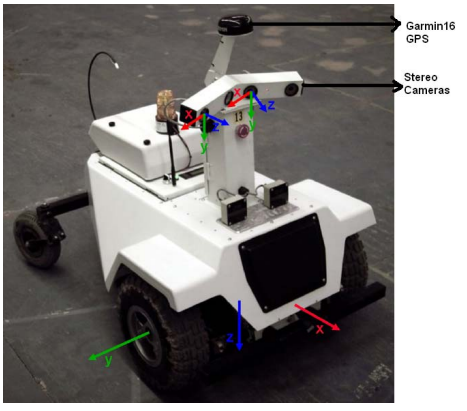
\includegraphics[scale=0.75]{Stereo}
\caption{A picture of the robot used in the work of Agrawal et al., which employs stereo cameras with GPS for localization. Image source: http://www.ai.sri.com/~agrawal/icpr06.pdf}
\end{figure}


\par
In our work, we propose to use neural networks to serve the role of a perceptual model. With enough training data, we believe that neural networks would be able to learn the invariant features of a map, which would allow them to be robust to different lighting and wheather conditions like point cloud methods as well as robust to variance in the set of objects in the environment like SIFT and SURF feature vectors. Furtheremore, CNNs do not require one to perform any feature engineering on the data, which not only cuts down development time, but may also make our methods robust to different environments which may have very different types of differentiating features. 
\begin{figure}[h]
\centering
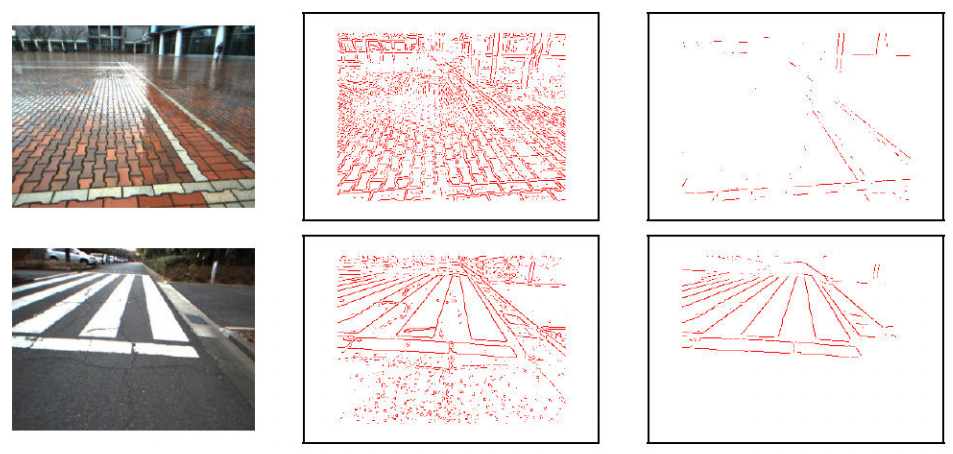
\includegraphics[scale=0.25]{point_clouds}
\caption{Point clouds generated by Irie et al. on their data set for localization using stereo cameras. Image source: $http://www.furo.org/irie/stereo_localization_iros10.pdf$}
\end{figure}

Valgren et al. instead propose to use SIFT and SURF features for image matching \cite{valgren2007sift}. In their work, they generate SIFT \cite{sift} and SURF\cite{surf} feature vectors for the images collected by their robot and use nearest neighbor approaches to match them to images in their training data. 

\begin{figure}[h]
\centering
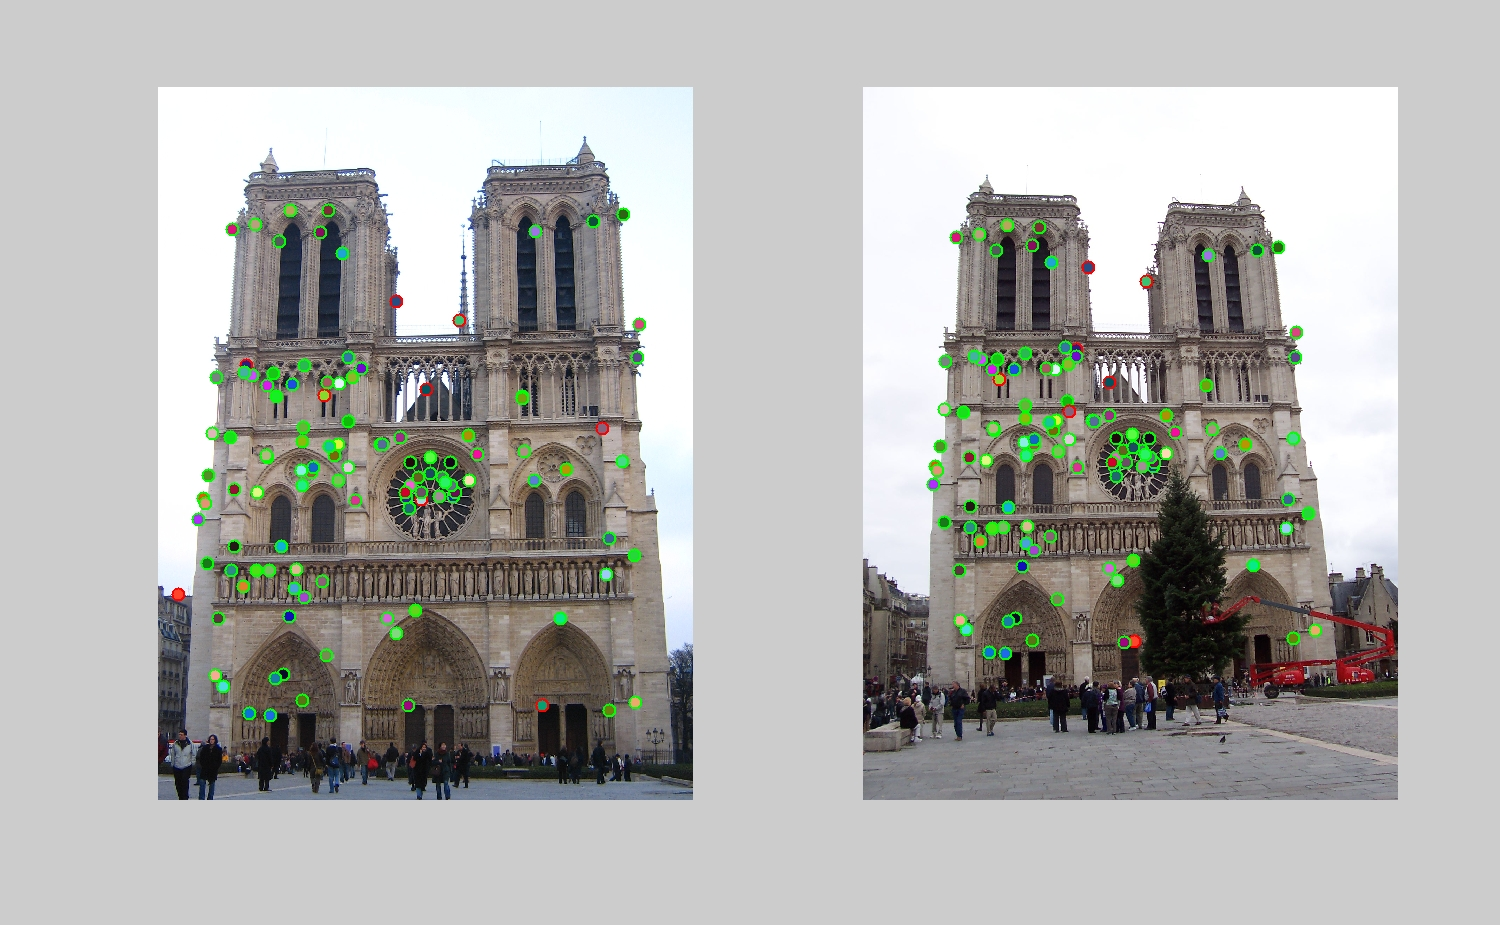
\includegraphics[scale=0.15]{sift}
\caption{An example of SIFT features generated for an image. Both SIFT and SURF generate feature vectors for images by finding key points such as edges, corners, or other areas where certain image gradients are higher. Image source: http://cs.brown.edu/courses/cs143/results/proj2/valayshah/}
\end{figure}


\section{Methodology}

\subsection{Data Set}
A roughly 280 meter path was chosen for use as a map for testing our particle filter. This path was traversed a total of 19 times at different times of day in order to capture as much variability in daylight as possible. Through each run, data from all robot sensors was collected (e.g. GPS, cameras, wheel odometry, etc.).  

\begin{figure}[h]
\centering
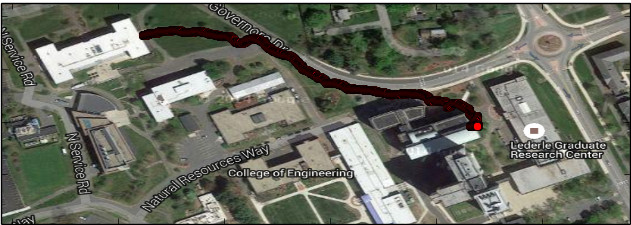
\includegraphics[scale=0.5]{map}
\caption{A satellite image of the map used in our data set. The red map shows the path traversed by the robot during data collection. Image source: https://www.google.com/maps}
\end{figure}

\subsection{Particle Filter Algorithm and Visualizer}
For our particle filter implementation, internal wheel odometry sensors were used to approximate trajectory in our motion model. Additionally, a GPS perceptual model was integrated in order to test the efficacy of the algorithm while the visual perceptual model was being developed. 
\par
In order to effectively use GPS for localization, the latitudinal and longitudinal variances, $\sigma _{lon}^2$ and $\sigma _{lat}^2$, for the Jackal's GPS were approximated experimentally by collecting readings from a set of three marked places five different times. Using these values, the following loss function was constructed:
$$
f(x_e,y_e,x_g,y_g)= \frac{1}{\sigma _{long}^2 + e^{|x_e-x_g|}}\cdot \frac{1}{\sigma _{lat}^2 + e^{|y_e-y_g|}}
$$
Where $x_e$ and $y_e$ are position estimates and $g_x$ and $g_y$ are GPS position readings. This function was then used in order to assign a weight to each particle in the weighing step of the algorithm, where a greater distance from the GPS reading results in a lower weight being assigned.
\par
In order to be able to qualitatively evaluate the particle filter implementation, the CMU Cobot \cite{cobot} localization visualizer was integrated into the system. Using the Cobot visualization library, the particle filter visualizer may take a log of saved sensor data from our data set and recreate it visually, effectively allowing the user to replay a run along the map. 

\begin{figure}[h]
\centering
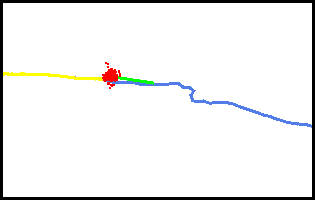
\includegraphics[scale=0.70]{particle_filter_visual}
\caption{A visualization of the particle filter using GPS. The blue path denotes the set of all GPS readings while the yellow path denotes the readings already given to the robot. The red dots represent the particle distribution and the green line, stemming from the particle cloud, represents the robot's pose.}
\end{figure}

\subsection{Neural Perceptual Model}
In order to effectively use cameras as sensors, a method that can work directly with raw RGB information with as little preprocessing as possible is desirable. CNNs are a well known tool that has been previously used with raw image data for a variety of machine learning tasks, particularly in object recognition. 
\par
Through a series of convolution operations on the image data, CNNs are able to extract higher level features from images such as edges and partial objects, features which we believe will prove effective in differentiating pictures taken at different locations from each other. 
\par
To this end, a pre-trained model of the AlexNet CNN architecture \cite{AlexNet}, which won the 2012 ImageNet Large Scale Visual Recognition Competition (ILSVRC), is used in order to extract higher level features from the images in our data set. Rather than use the entire network for our classification task, these feature vectors are used with a variety of different classification algorithms (e.g K-Nearest Neighbors, SVNs, etc.) in order to determine an effective model for localization.  

\begin{figure}[h]
\centering
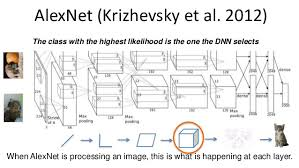
\includegraphics[scale=0.70]{alexnet}
\caption{The AlexNet CNN architecture. At each layer features are extracted, starting from lower level features such as edges and colors, growing in abstraction to feature types such as partial objects. Image source: http://www.cc.gatech.edu/~hays/compvision/proj6/}
\end{figure}



\section{Results}

\subsection{Particle Filter}

After completion, the particle filter implementation was evaluated qualitatively in a variety of settings in order to ensure that it behaved as would be expected in a variety of conditions. 
\par
As a sanity check, the filter was first tested on synthetic odometry data which gave readings denoting only forward movement on the x-axis. One such run with only odometry readings may be seen in figure \ref{odometry_error}, as would be expected, the error models developed for the Jackal result in some uncertainty in trajectory at each time step, which is reflected by the distribution of particles. Without any correction from other senors, the distribution can be seen to quickly diverge, denoting an ever growing level of uncertainty of the robot's true pose. 

\begin{figure}[h]
\centering
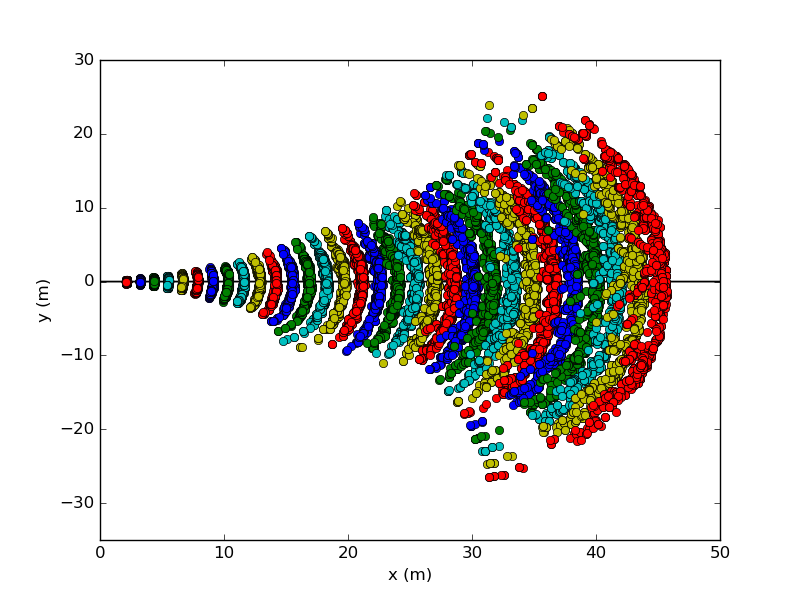
\includegraphics[scale=0.60]{NO_GPS}
\caption{A visualization of the particle filter using only wheel odometry with synthetic data denoting forward movement. As may be seen, without any correction from a perceptual model, the uncertainty of the model grows quickly over time. }
\label{odometry_error}
\end{figure}

Following this, synthetic GPS data was added to this evaluation by giving a GPS reading with coordinates matching the true location of the robot in the data at each time step. As may be seen in figure \ref{with_gps}, the uncertainty of the run is greatly mitigated, with the distribution of particles clearly remaining within the GPS roughly 10 meter radius of uncertainty. 

\begin{figure}[h]
\centering
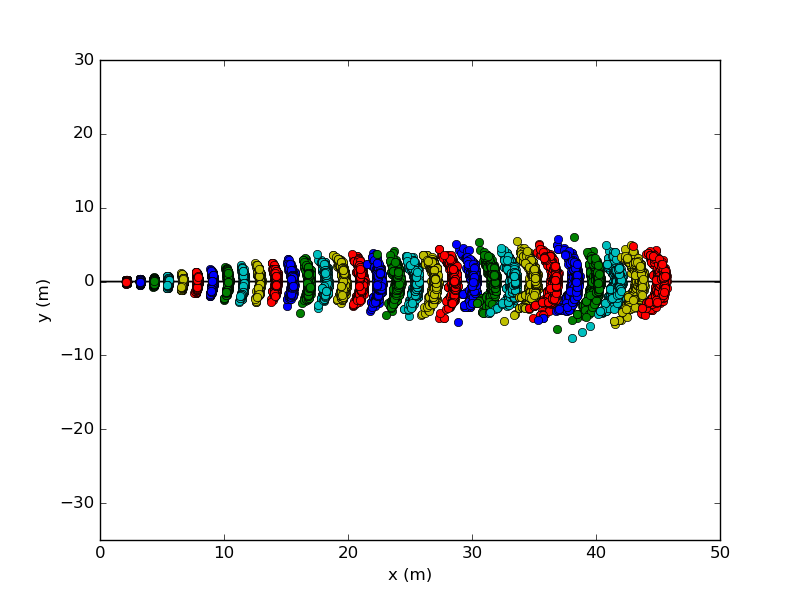
\includegraphics[scale=0.60]{With_GPS}
\caption{A visualization of the particle filter using wheel odometry and GPS with synthetic data denoting forward movement. It may be observed that the distribution of particles is maintained within the GPS radius of uncertainty. }
\label{with_gps}
\end{figure}

\subsection{Visual Classification}

Because classification algorithms operate on a discrete set of possible values, it is necessary to discretize the continuous space of GPS readings for our task. In order to do this, K-Means clustering was used on our training data in order to generate 100 clusters along our map, which served as the set of possible classes which images could be labeled with. 
\par 

\begin{figure}[h]
\centering
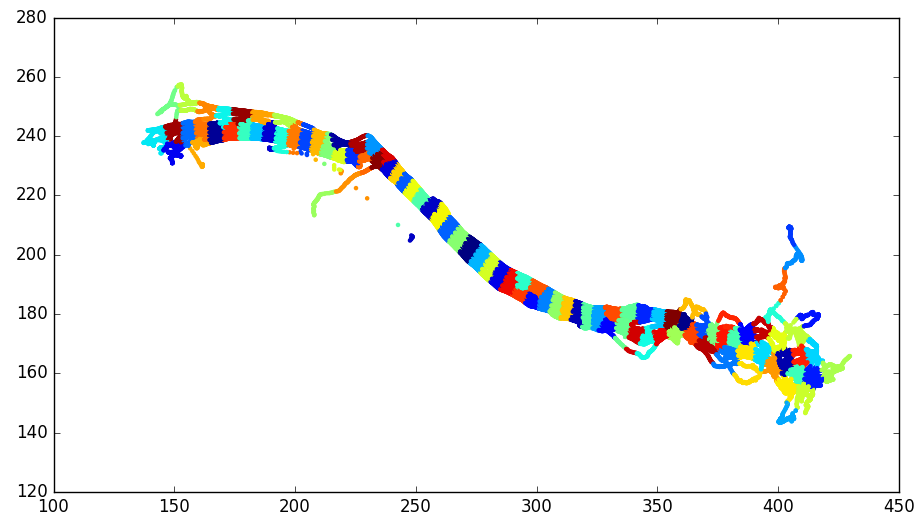
\includegraphics[scale=0.5]{clustering}
\caption{A visualization of the classes generated on our dataset through K-Means clustering using cartesian coordinates in meters. Each colored patch denotes a different class, the average distance of GPS points in our data set to the nearest cluster center was 5.53 meters.}
\label{clustering}
\end{figure}

For a preliminary evaluation of our methods, a K-Nearest Neighbor classifier was trained using 18 runs from our data set, and the 19th was used for testing. For evaluation, feature vectors were extracted for our test set from a variety of layers of the AlexNet CNN, which were then run through the classifier. The classification accuracy of this experiment performed for each layer may be seen in figure \ref{classification_results}. From these results, it was determined that the fifth pooling should be used.  

\begin{figure}[h]
\centering
\begin{tabular}{| c | c |}
\hline
\textbf{Layer} & \textbf{Accuracy} \\
\hline
Fully Connected 7 & 0.31 \\ 
Fully Connected 6 & 0.38 \\
Pooling 5 & 0.42 \\
Convolutional 4 & 0.41 \\
Convolutional 3 & 0.35 \\
Pooling 2 & 0.41 \\
Pooling 1 & 0.37 \\
\hline
\end{tabular}
\caption{The accuracy of the K-Nearest Neighbor classification on feature vectors pulled from a variety of layers of the AlexNet CNN. }
\label{classification_results}
\end{figure}

\subsection{Error Analysis}

Given the low accuracy of our classification results, error analysis was conducted in order to determine the possible sources of error. 

\begin{figure}[h]
\centering
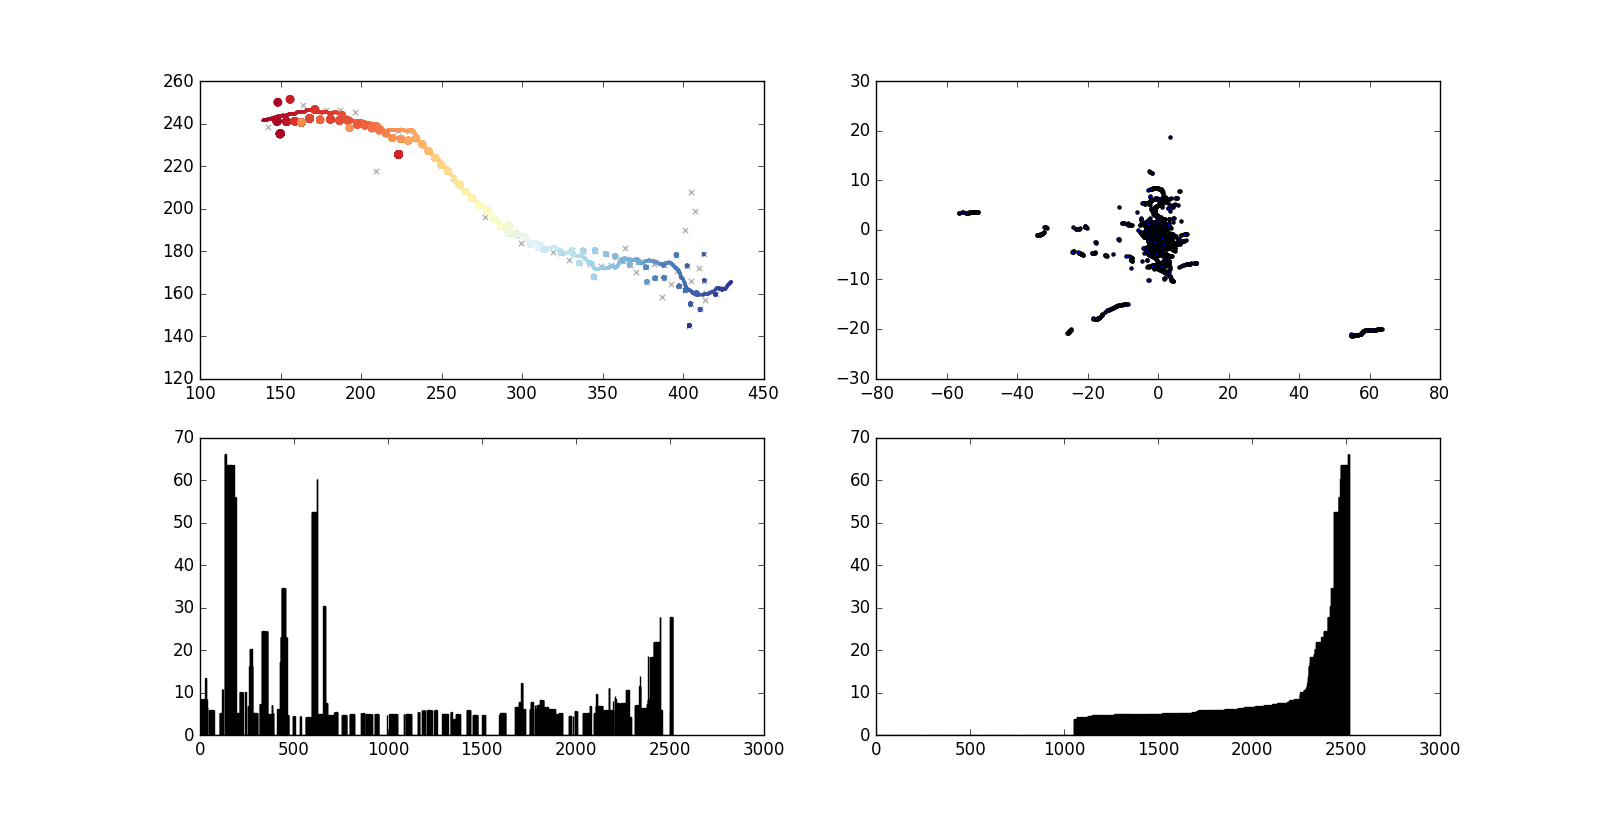
\includegraphics[scale=0.25]{error_pool5}
\caption{Visualizations of error from the fifth pooling layer. \textit{Top Left)} The continuous multi-colored path represents the ground truth path taken in the test run. The location of colored dots represent the location they were classified under, while the color corresponds to the true classification on the path.  \textit{Top Right)} The distance between labels assigned to images and the location of their true label. This graphic shows that the majority of error was kept within a 10 meter radius. \textit{Bottom Left)} Another measure of error between assigned labels and their true class. From this it may be inferred that the greatest error occurred towards the beginning of the run and at the end. \textit{Bottom Right)} The same measure as the bottom left, sorted by error magnitude. Like the top right, this graphic implies that the majority of error was kept within a 10 meter distance.}
\label{error_graphs}
\end{figure}

Figure \ref{error_graphs} shows the results from some error analysis that was conducted. In general, it was found that the majority of misclassified images had been labeled with a class that was within 10 meters from the correct class, which suggests that the model was able to learn general locations relatively effectively. It may be seen that there were only certain areas with much higher error. 
\par
In order to get a clearer idea of which parts of the map the model failed in, a confusion matrix was constructed
\begin{figure}[h]
\centering
\includegraphics[scale=0.08]{heatmap_knn}
\caption{Visualizations of error from the fifth pooling layer. \textit{Top Left)} \textit{Top Right)} \textit{Bottom Left)} \textit{Bottom Right)}}
\label{confusion_matrix}
\end{figure}
which visualized the correlation between the assigned and true labels for the images. Looking at the result of this analysis in figure \ref{confusion_matrix}, it may be seen that the model performed well throughout most of the map, only faltering at either end, with the error being particularly pronounced at the bottom right of the matrix. By once more looking back at the clusters in figure \ref{clustering}, it may be observed that the clusters are very consistent throughout the middle of the track, and diverge much more at the ends, particularly at the bottom right end of the map. 

\section{Discussion and Future Work}

Because the same path was followed each time data was collected on our map, it is clear that the divergence in clustering classes is due to GPS error. This variance in classes in parts of our map proved to cause too adverse and effect on our results. Because of this inconsistency found within the GPS, it was determined that a different method of collecting ground-truth locations for images is necessary. 
\par
Another factor that proved too problematic in the methodology was the data collection step. Because neural networks need large amounts of data to train, images were collected from many runs, a process which took approximately a week for a 280 meter path. Because a long-term goal of the project is to be able to create a map of the entire campus, this method of collecting data would prove to be too time consuming, necessitating different methods. 
\par
For the reasons deleniated above, it was determined that a first alternative to explore would be the use of satellite imagery. We would like to explore methods of finding the correspondence between imaegs taken from the ground and images taken over satellite. Because GPS coordinates of satellite imagery may be easily determined, we believe that finding a time-effective method of mapping ground images to their respective patch of a satellite image would prove fruitful for our goals. 

\section{conclusion}

A particle filter was implemented for use with the Jackal robot's GPS and internal wheel odometry sensors. Furtheremore, the filter was integrated with visualization software which allowed for a qualitative analysis of the algorithm. Preliminary methods for developing a visual perceptual model using CNNs was explored, and some problems were found with the initial methodology. For future work, we plan on aleviating these problems in order to have a robust visual perceptual model which will allow for outdoor localization around campus. 

\bibliographystyle{plain}
\bibliography{bibliography}

\addtolength{\textheight}{-12cm}   % This command serves to balance the column lengths
                                  % on the last page of the document manually. It shortens
                                  % the textheight of the last page by a suitable amount.
                                  % This command does not take effect until the next page
                                  % so it should come on the page before the last. Make
                                  % sure that you do not shorten the textheight too much.

%%%%%%%%%%%%%%%%%%%%%%%%%%%%%%%%%%%%%%%%%%%%%%%%%%%%%%%%%%%%%%%%%%%%%%%%%%%%%%%%



%%%%%%%%%%%%%%%%%%%%%%%%%%%%%%%%%%%%%%%%%%%%%%%%%%%%%%%%%%%%%%%%%%%%%%%%%%%%%%%%



%%%%%%%%%%%%%%%%%%%%%%%%%%%%%%%%%%%%%%%%%%%%%%%%%%%%%%%%%%%%%%%%%%%%%%%%%%%%%%%%




\end{document}
